\section{Metodologías}
\subsection{Metodología de Diseño}

El desarrollo del mecanismo se llevó a cabo mediante una metodología  basada en reuniones periódicas del equipo, durante las cuales se evaluaron diferentes alternativas de diseño mecánico, electrónico y estructural. Cada decisión fue sustentada mediante criterios técnicos y posteriormente validada mediante votación entre los integrantes del grupo.

Inicialmente se analizó el mecanismo propuesto por el docente, identificando las variables cinemáticas y dinámicas involucradas, así como los requerimientos de medición necesarios para la adquisición de datos experimentales.

\subsubsection{Selección del sistema de medición}

Con el objetivo de registrar las aceleraciones presentes en el mecanismo, se evaluaron dos alternativas de sensores inerciales: el MPU6050 y el BMI160. La comparación se realizó considerando aspectos relevantes para la adquisición experimental de datos dinámicos.

\begin{table}[H]
\centering
\caption{Comparación entre sensores inerciales.}
\begin{tabularx}{\columnwidth}{|X|c|c|}
\hline
\rowcolor{gray!20}
Característica & MPU6050 & BMI160\\
\hline
Consumo energético & Alto & Bajo\\
Resolución acelerómetro & 14 bits & 16 bits\\
Resolución giroscopio & 16 bits & 16 bits\\
Tamaño FIFO & 512 bytes & 1024 bytes\\
Ruido de medición & Mayor & Menor\\
Modos de bajo consumo & Limitados & Avanzados\\
Tamaño físico & Mayor & Menor\\
\hline
\end{tabularx}
\end{table}

Tras la discusión técnica y posterior votación del equipo, se seleccionó el sensor BMI160 debido a su menor consumo energético, mayor resolución y mejor desempeño en la adquisición de señales dinámicas

\subsubsection{Selección del mecanismo de accionamiento}

Posteriormente se analizaron tres posibles mecanismos para generar el movimiento vertical de los puntos A y C: sistema tornillo-tuerca, sistema cremallera-piñón y cilindro neumático.


\begin{table}[H]
\centering
\caption{Evaluación del sistema tornillo-tuerca.}
\begin{tabularx}{\columnwidth}{|X|X|}
\hline
\rowcolor{green!20}
Ventajas & Desventajas\\
\hline
Relación de transmisión precisa y fácilmente modelable &
Presencia de fricción significativa\\
\hline
Alta capacidad de carga axial &
Requiere lubricación periódica\\
\hline
Buena repetibilidad del movimiento &
Posibles holguras axiales\\
\hline
Integración sencilla con motores paso a paso &
Velocidad lineal limitada\\
\hline
\end{tabularx}
\end{table}


\begin{table}[H]
\centering
\caption{Evaluación del sistema cremallera-piñón.}
\begin{tabularx}{\columnwidth}{|X|X|}
\hline
\rowcolor{green!20}
Ventajas & Desventajas\\
\hline
Conversión directa entre movimiento rotacional y lineal &
Presencia de backlash\\
\hline
Alta velocidad de desplazamiento &
Menor precisión de posicionamiento\\
\hline
Fabricación relativamente sencilla &
Mayor desgaste de los dientes\\
\hline
Mantenimiento reducido &
Requiere alineación precisa\\
\hline
\end{tabularx}
\end{table}
\begin{figure}[H]
    \centering
    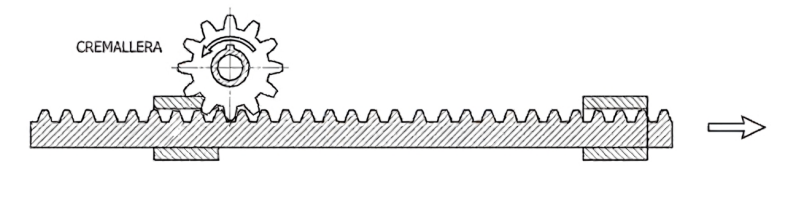
\includegraphics[width=\columnwidth]{img/cremallera.png}
    \caption{Alternativa piñon-cremallera}
    \label{fig:prototipo}
\end{figure}


\begin{table}[H]
\centering
\caption{Evaluación del sistema neumático.}
\begin{tabularx}{\columnwidth}{|X|X|}
\hline
\rowcolor{green!20}
Ventajas & Desventajas\\
\hline
Alta relación potencia-peso &
Modelado dinámico complejo\\
\hline
Movimiento suave &
Posicionamiento menos preciso\\
\hline
Amplio uso industrial &
Requiere compresor y accesorios\\
\hline
&
Mayor costo de implementación\\
\hline
\end{tabularx}
\end{table}

\begin{figure}[H]
    \centering
    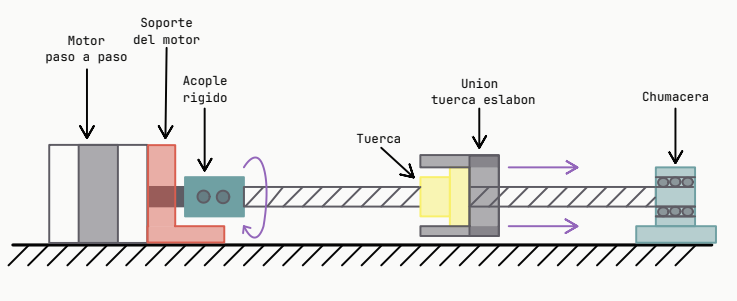
\includegraphics[width=\columnwidth]{img/tornillo.png}
    \caption{Alternativa tornillo-tuerca}
    \label{fig:prototipo_tornillo}
\end{figure}


Luego de analizar las tres alternativas y considerando criterios de precisión, facilidad de fabricación, costo y simplicidad de modelado, el equipo seleccionó el sistema tornillo-tuerca como mecanismo de accionamiento principal.

\subsubsection{Selección del material de las barras}

Para la fabricación de las barras del mecanismo se evaluaron diferentes materiales considerando criterios de masa, resistencia mecánica, facilidad de manufactura, disponibilidad comercial y costo.

\begin{table}[H]
\centering
\caption{Resultados de la votación para selección de material.}
\begin{tabularx}{\columnwidth}{|X|c|}
\hline
\rowcolor{gray!20}
Material & Votos\\
\hline
PVC & 2\\
Impresión 3D & 0\\
Acero & 0\\
Aluminio (varilla) & 3\\
Perfil de aluminio & 1\\
Acrílico & 3\\
\hline
\end{tabularx}
\end{table}

\begin{table}[H]
\centering
\caption{Evaluación técnica del aluminio.}
\begin{tabularx}{\columnwidth}{|X|X|}
\hline
\rowcolor{green!20}
Ventajas & Desventajas\\
\hline
Baja densidad &
Costo superior al PVC\\
\hline
Buena relación resistencia-peso &
Menor resistencia absoluta que el acero\\
\hline
Resistencia a la corrosión &
\\
\hline
Facilidad de mecanizado &
\\
\hline
Disponibilidad comercial &
\\
\hline
\end{tabularx}
\end{table}

Finalmente se seleccionó el aluminio debido a su favorable relación entre masa y resistencia mecánica, así como su apariencia profesional.

\subsubsection{Componentes seleccionados}

Una vez definidas las alternativas de diseño, se estableció la lista preliminar de componentes necesarios para la construcción del prototipo.

\begin{table}[H]
\centering
\caption{Componentes principales del sistema.}
\begin{tabularx}{\columnwidth}{|X|c|}
\hline
\rowcolor{gray!20}
Componente & Cantidad\\
\hline
Motor NEMA 17 & 2\\
Varilla roscada trapezoidal 8 mm & 2\\
Tuerca trapezoidal & 2\\
Guía lineal de aluminio & 2\\
Sensor BMI160 & 2\\
ESP32 & 1\\
\hline
\end{tabularx}
\end{table}

\subsubsection{Diseño asistido por computador}

El modelado tridimensional del sistema se desarrolló utilizando Autodesk Fusion 360. Esta herramienta permitió diseñar las piezas personalizadas, verificar interferencias geométricas y realizar el ensamblaje virtual previo a la fabricación física del mecanismo.

\subsection{Distribución de responsabilidades}

Con el fin de optimizar el desarrollo del proyecto, las actividades de diseño fueron distribuidas entre los integrantes del equipo.

\begin{table}[H]
\centering
\caption{Asignación de responsabilidades.}
\begin{tabularx}{\columnwidth}{|l|X|}
\hline
\rowcolor{gray!20}
Integrante & Actividad\\
\hline
David &
Diseño de uniones tuerca-varilla y soporte de sensores.\\
\hline
Sara &
Diseño de chumaceras y ensamblaje CAD.\\
\hline
Johel &
Diseño de la base y diagramas mecánicos.\\
\hline
Sergio &
Documentación en \LaTeX, rediseño del problema y soportes NEMA 17.\\
\hline
\end{tabularx}
\end{table}

\section{Descripción del prototipo seleccionado}

El prototipo desarrollado corresponde a la implementación física del mecanismo estudiado, compuesto por dos actuadores lineales ubicados en los puntos extremos y un sistema de barras articuladas que reproduce la configuración cinemática planteada inicialmente.



El movimiento vertical de los puntos A y C se genera mediante dos mecanismos independientes de tornillo-tuerca accionados por motores paso a paso NEMA 17. La rotación de cada motor se transforma en un desplazamiento lineal gracias a las varillas roscadas trapezoidales, permitiendo controlar la posición de los extremos del mecanismo con una relación geométrica conocida.

Las barras que conforman los eslabones móviles fueron fabricadas en aluminio, material seleccionado por su baja masa, adecuada rigidez estructural y facilidad de manufactura. Los puntos de unión se implementaron mediante articulaciones que permiten la rotación relativa entre los elementos, aproximando las condiciones ideales consideradas en el análisis teórico.

Para la adquisición de datos experimentales se incorporaron sensores inerciales BMI160, conectados a un microcontrolador ESP32 encargado de la lectura, procesamiento y transmisión de la información obtenida durante las pruebas. Esta instrumentación permite registrar las aceleraciones del mecanismo y compararlas posteriormente con los resultados obtenidos mediante el modelo dinámico.

Todos los componentes fueron montados sobre una base rígida (MDF). Adicionalmente, el ensamblaje completo fue modelado previamente en Autodesk Fusion 360 e Inventor, permitiendo verificar interferencias geométricas y validar el diseño antes de su fabricación.

\subsection{Principio de funcionamiento}

El funcionamiento del prototipo se basa en la conversión de movimiento rotacional a movimiento lineal mediante mecanismos tornillo-tuerca. Al girar los motores paso a paso, las tuercas acopladas a las varillas roscadas se desplazan verticalmente, generando el movimiento de los puntos A y C. Debido a la restricción impuesta por las barras articuladas, el punto B describe una trayectoria determinada por la geometría del mecanismo.